\section{Dynamics}
When drawing a \textbf{free body diagram}:
\begin{itemize}
	\item Draw all external forces acting only on the chosen system.
	\item Do not draw in the resultant force.
\end{itemize}

\subsection{Newton's Laws of Motion}
\begin{defn}{Newton's 1st Law of Motion}{}
A body at rest will remain at rest, a body in motion will remain in motion at constant velocity, \underline{in absence of external resultant force}. 
\end{defn} 

\begin{defn}{Newton's 2nd Law of Motion}{}
Rate of change of momentum is directly proportional to \underline{external} resultant force acting on it, and occurs in the direction of the external resultant force. 
\begin{equation} \sum \vb{F} = \dv{\vb{p}}{t} \end{equation}
(The constant of proportionality is found experimentally to be 1.)
\end{defn}

\begin{remark}
For questions, you will usually use the form $\displaystyle\sum\vb{F}=\frac{\Delta\vb{p}}{\Delta t}$.
\end{remark}

\begin{remark}
Using product rule, we have 
\[ \sum \vb{F}=\dv{\vb{p}}{t}=\dv{(m\vb{v})}{t}=m\dv{\vb{v}}{t}+\vb{v}\dv{m}{t} \]
Hence $\sum F = ma$ holds only when mass is constant.
\end{remark}

\begin{remark}
Resultant force and acceleration act in the same direction.
\end{remark}

\begin{defn}{Newton's 3rd Law of Motion}{}
When body A exerts a force on body B, body B exerts force of the \underline{same type}, \underline{equal in magnitude}, \underline{opposite in direction} on body A. 
\begin{equation} \vb{F}_{AB} = - \vb{F}_{BA} \end{equation}
\end{defn}

\begin{defn}{Inertia}{}
Reluctance of a body to change its state of rest or uniform motion in a straight line, due to mass. 
\end{defn} 
\begin{remark}
Mass is the property of a body which resists change in motion (inertia).
\end{remark}
\pagebreak

\subsection{Linear momentum and its conservation}
\begin{defn}{Linear momentum}{}
Product of a body's mass and velocity. 
\begin{equation}
\vb{p} = m\vb{v}
\end{equation}
\end{defn} 

\begin{defn}{Impulse}{}
Product of a constant force $F$ and the time interval $t$ for which the constant force acts. 
\begin{equation} 
\vb{J} = \int\vb{F}\dd{t} = \vb{F}_{\mathrm{avg}} \Delta t \end{equation}
\end{defn} 
Graphically, impulse is the area under a force-time graph. 

For collisions, the area under both graphs (representing impulse of force on each object by the other) must be the same, as linear momentum is conserved.

\begin{defn}{Impulse-Momentum Theorem}{}
The impulse applied to a body is equal to the body's change in momentum.
\begin{equation}
\vb{J} = \Delta\vb{p} = \vb{p}_f-\vb{p}_i
\end{equation}
\end{defn} 

\begin{defn}{Principle of Conservation of Momentum}{}
Total momentum of a \underline{system} of bodies is constant, provided \underline{no external resultant force} acts on the system.
\begin{equation}
\sum \vb{F} = 0 \implies \vb{J} = 0 \implies \vb{p}_i=\vb{p}_f
\end{equation}
\end{defn} 
\pagebreak

\subsection{Collisions}
\subsubsection{1D collision}
\textbf{Head-on collision}: contact forces between the two objects act radially along a line joining their centres of mass, with no component tangential to their circumference.

Types of collisions:
\begin{enumerate}
\item \textbf{Elastic} collision
\item \textbf{Inelastic} collision
\item \textbf{Perfectly inelastic} collision (coalescence)
\item \textbf{Super elastic} collision
\end{enumerate}

Problem solving:
\begin{itemize}
\item \textbf{Linear momentum} is always conserved for every type of collision (except super elastic collisions). \[ m_1 u_1 + m_2 u_2 = m_1 v_1 + m_2 v_2 \]

\item \textbf{Kinetic energy} is conserved for elastic collisions, from which we can derive: relative speed of approach = relative speed of separation (r.s.a. = r.s.s.) \[ u_1-u_2 = v_2-v_1 \] 
 
Kinetic energy is not conserved for inelastic collisions, is lost to surroundings, hence relative speed of approach $>$ relative speed of separation (r.s.a $>$ r.s.s.) \[ u_1-u_2 > v_2-v_1 \]

Kinetic energy is not conserved for super elastic collisions, is gained due to stored forms of energy (potential energy) e.g. bullet shot at a stationary hand grenade and a hand grenade explodes, where the additional energy comes from chemical energy of explosives stored in the grenade.
\end{itemize}

\subsubsection{2D collision}
\textbf{Oblique collision}: 
If an object obliquely collides with another stationary object of equal mass, they travel off at an angle of 90° relative to one another (for elastic collision).
\pagebreak

\subsection{Problems}
\begin{prbm}[Stacked ball drop]
Two balls are dropped to the floor, with the lighter ball atop the heavier one. The balls collide approximately elastically with each other and with the floor. The observation is the small ball flies up to a height higher than it was dropped.
\end{prbm}
\begin{solution} \ {\\}
\begin{figure}[H]
    \centering
    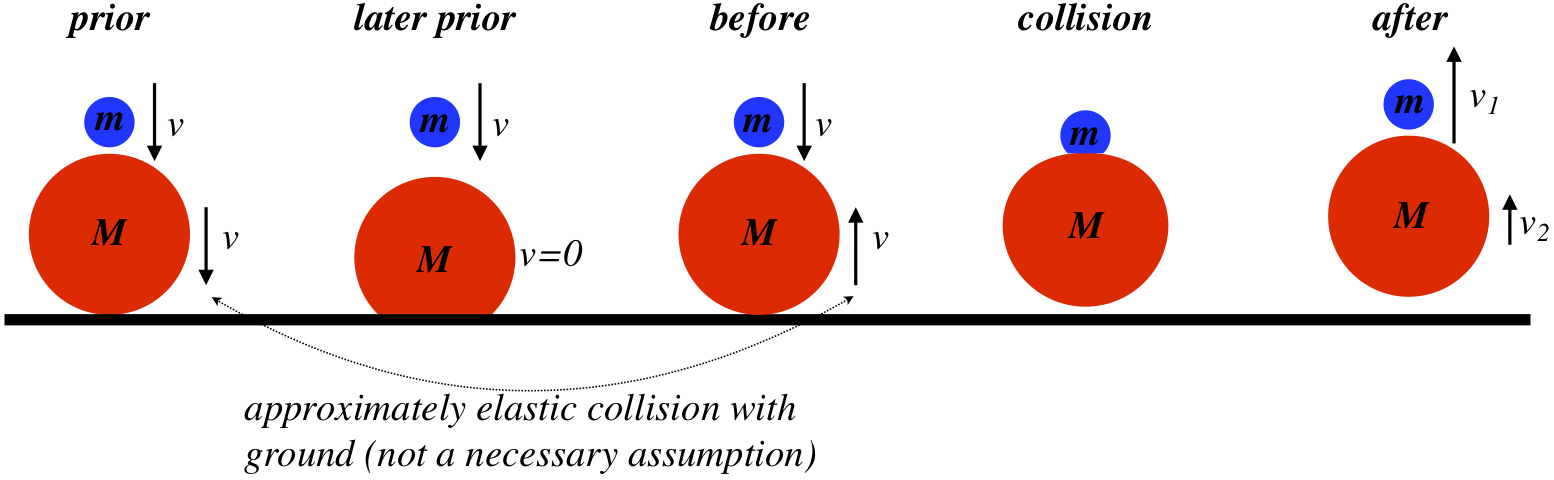
\includegraphics[width=15cm]{images/Stacked_balls.png}
\end{figure}

Conservation of momentum gives us 
\[ Mv - mv = mv_1 + Mv_2 \]
Conservation of kinetic energy gives us 
\[ \frac{1}{2}mv^2 + \frac{1}{2}Mv^2 = \frac{1}{2}m{v_1}^2 + \frac{1}{2}M{v_2}^2 \]

We can now solve for $v_1$ and $v_2$ in terms of $v$, which we can determine from the height that the balls are dropped from.
\[ v_1=\brac{\frac{3M-m}{M+m}}v \]
\[ v_2=\brac{\frac{M-3m}{M+m}}v \]

We see that the small ball must rise to a height greater than that from which it was dropped, because the fraction in front of $v$ is always greater than 1.
\end{solution}
\pagebreak

\begin{prbm}
A flatcar of mass $m$ moves towards the right from rest due to a constant horizontal force $F$. At the same time, sand spills on the flatcar from a stationary hopper at a constant rate of $\mu\:\unit{kg.s^{-1}}$. 

\begin{figure}[H]
    \centering
    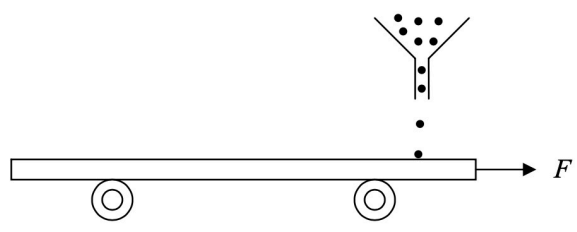
\includegraphics[width=10cm]{images/Sand_car.png}
\end{figure}

What is the dependence of the velocity $v$ of the flatcar with respect to time $t$, assuming that friction is negligibly small?
\end{prbm}

\begin{solution}
Recall that force is the rate of change of momentum. 
\[ F=\dv{p}{t} \implies \Delta p=F\Delta t \]
The momentum of the flatcar due to from the additional mass of the sand which is $\mu t$, as well as from the increase in velocity $v$. 

At time $t = 0$, $p = 0$. At time $t = t$, the momentum is 
\[ p=(m+\mu t)v=Ft \]

Hence we get \[ \boxed{v=\frac{Ft}{m+\mu t}} \]
\end{solution}
\pagebreak